\documentclass[a4paper]{article}
\usepackage{fullpage}
\usepackage[latin 1]{inputenc}
\usepackage[francais]{babel}
\usepackage{graphicx}
\usepackage{listings}
\usepackage{color} 
\usepackage{enumerate}
\usepackage{amsfonts}
\usepackage{amssymb}
\usepackage{amsmath}
\usepackage{wasysym}

\usepackage[usenames,dvipsnames]{pstricks} % pour inclure le schéma relationnel
\usepackage{epsfig}
\usepackage{pst-grad} % For gradients
\usepackage{pst-plot} % For axes

%%%%% Marges %%%%%
\addtolength{\textwidth}{0cm}
\addtolength{\oddsidemargin}{-0.8cm}
\textheight=21cm % longueur utile de la page
\topmargin=0cm % marge haute
\headsep=40pt % séparation 40 points entre entête et texte
\footskip=15pt % idem séparation pied de page

%%%%% Entetes et Enpieds de pages %%%%%
\usepackage{fancyhdr}
\pagestyle{fancy}
\lhead{\footnotesize{\textit{Bruno Bassac, Geoffrey Graveaud, Fabien
Kuntz}}}
\rhead{\footnotesize{\textit{Bases de donn\'ees avanc\'ees - Michel
Prudence, Christian R\'etor\'e}}}

%%%%% Numrotation sections %%%%
\setcounter{secnumdepth}{3}
\setcounter{tocdepth}{3}

%%%%% Types enumerate %%%%%
\let\enumeratesav\enumerate
\let\endenumeratesav\endenumerate

\renewcommand{\labelenumi}{\indent-}
\renewcommand{\labelenumii}{\indent$\bullet$}
\renewcommand{\labelenumiii}{\indent$\star$}
\renewcommand{\labelenumiv}{\indent\_}

%%%%% Titre %%%%%
\newlength{\larg}
\setlength{\larg}{14.5cm}

%%%Zone de Code%%%
\definecolor{gray}{gray}{0.86}  

\lstset{numbers=left, tabsize=2, frame=single, breaklines=true,
basicstyle=\ttfamily,numberstyle=\tiny\ttfamily, framexleftmargin=13mm,
backgroundcolor=\color{gray}, xleftmargin=14mm} 

\newsavebox{\fmbox}
\newenvironment{fmpage}[1]{\begin{lrbox}{\fmbox}\begin{minipage}{#1}}{\end{minipage}\end{lrbox}\fbox{\usebox{\fmbox}}}


%%%%%%          %%%%%%
%%%%%% DOCUMENT %%%%%%
%%%%%%          %%%%%%


\begin{document}


%%%%% Page de présentation %%%%%
\thispagestyle{empty}

\setlength{\unitlength}{1in}



\begin{flushright}
 \noindent {\rule{\larg}{0.5mm}}
\end{flushright}
\vspace{7mm}
\begin{flushright}
 \Huge{\bf Bases de donnes avanc\'ees} \\
 \Huge{\bf Projet} \\
 ~\\
 \huge{Gestion d'une agence de voyage}\\
\end{flushright}
\vspace{7mm}
\begin{flushright}
 {\rule{\larg}{0.5mm}}
\end{flushright}
\vspace{2mm}
\begin{flushright}
 \large{\bf Professeurs : Michel Prudence, Christian R\'etor\'e} \\
 ~\\
 \large{Master 2 Informatique}\\
 ~\\

\begin{figure}[ht]
\begin{center}
%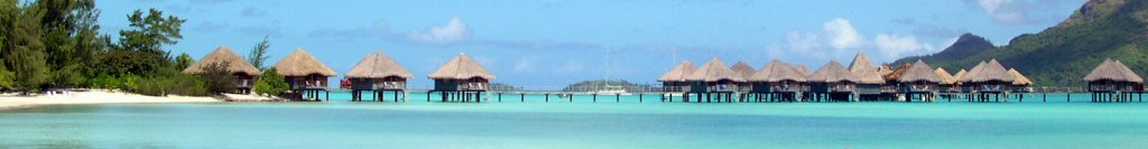
\includegraphics[height=8cm]{fond.eps}
\end{center}
\end{figure}



 \large{Bruno Bassac, Geoffrey Graveaud, Fabien Kuntz}
{\rule{\larg}{0.5mm}}
\end{flushright}

\newpage

\addtolength{\oddsidemargin}{1cm}

%%%%% Table des matières %%%%%
\thispagestyle{empty}
\tableofcontents
\newpage

\setcounter{page}{1}


%%%%%%              %%%%%%
%%%%%% ZONE DE CODE %%%%%%
%%%%%%              %%%%%%

\section{Pr\'esentation du projet}
%pr\'esentation/introduction
%les objectifs recherch\'es
Le but du projet \'etait de cr\'eer une base de donn\'ees et une interface graphique pour aider \`a la gestion d'une agence de voyage. Cette application a \'et\'e d\'evelopp\'ee sur une base \textit{Oracle} pour stocker les donn\'ees de l'agence et l'interface Client/Utilisateur a \'et\'e d\'evelopp\'ee via des outils PHP. L'interface Client doit \^etre capable de pr\'esenter les offres de l'agences, les disponibilit\'es mais \'egalement de permettre \`a l'utilisateur des saisies en ligne selon ses voeux. Les donn\'ees saisies seront ensuite enregistr\'ees dans la base et accessibles au gestionnaire de la base.


\section{Cahier des charges}
%Les \'el\'ements qui doivent \^etre mis en avant : information, produits, services...)
Nous pr\'esentons ici les \'el\'ements impos\'es pour la cr\'eation de la base de donn\'ees.

L'agence doit g\'erer 50 destinations, dans 10 pays du monde et offre les prestations suivantes:
\begin{itemize}
\item 5 destinations par pays
\item 4 cat\'egories d'h\^otel
\item 3 circuits diff\'erents par destination
\end{itemize}

Les prestations sont calcul\'ees de la fa\c{c}on suivante:
\begin{itemize}
\item 1 tarif adulte + 1 tarif enfant par destination pour le vol
\item 1 tarif par type d'h\^otel pour chambre une personne, et pour chambre double
\item 1 tarif par circuit en fonction de la longueur du s\'ejour.
\end{itemize}

Les s\'ejours seront de 10 jours ou 21 jours, des tarifs pr\'ef\'erentiels seront accord\'es sur les p\'eriodes de basse saison, p\'eriode de f\^etes, $\ldots$

Chaque mois, il y a 4 d\'eparts par destination. Pour chaque d\'epart, il y a 100 personnes.

En plus, des tables cr\'eees pour la base de donn\'ees, il faudra g\'erer une table client et une table facturation. Dans la table facturation, il faudra une ligne pour chaque prestation: Avion, H\^otel, tarif enfant, r\'eductions, $\ldots$. Il faudra reconstituer le total de chaque facture par client. La table facturation nous servira donc \'a l'\'edition de la facture.

Une ligne de facturation est li\'ee \'a un client avec une adresse et un montant par prestation. A noter que la	facturation est un mod\`ele \'a part enti\`ere, via ce mod\`ele on doit \^etre capable de conna\^itre nos clients: age, classe sociale, destinations pr\'ef\'er\'ees, investissement moyen. Il est \'egalement demand\'e de conserver un historique en ligne de la partie comptable sur 10 ans.

L'agence veut pouvoir faire des statiqtiques sur les destinations les plus demand\'ees. Il faudra \'egalement g\'erer le chiffre d'affaire global et par destination, par mois et par an.

Enfin l'interface utilisateur devra \^etre capable d'afficher la liste des diff\'erents circuits, avec des options sur le type d'h\^otel et le choix de la chambre(chambre simple ou double).


\section{Organisation relationelle de la base de donn\'ee}

\scalebox{0.9} % Change this value to rescale the drawing.
{
\begin{pspicture}(0,-7.2871876)(18.88,7.2471876)
\definecolor{color66}{rgb}{0.0196078431372549,0.11372549019607843,0.9647058823529412}
\definecolor{color67}{rgb}{0.984313725490196,0.03137254901960784,0.03137254901960784}
\definecolor{color68}{rgb}{0.043137254901960784,0.10980392156862745,0.9411764705882353}
\definecolor{color69}{rgb}{0.027450980392156862,0.047058823529411764,0.9764705882352941}
\definecolor{color70}{rgb}{0.9803921568627451,0.054901960784313725,0.054901960784313725}
\definecolor{color71}{rgb}{0.9607843137254902,0.054901960784313725,0.03529411764705882}
\definecolor{color72}{rgb}{0.9882352941176471,0.043137254901960784,0.043137254901960784}
\definecolor{color73}{rgb}{0.027450980392156862,0.058823529411764705,0.9725490196078431}
\definecolor{color74}{rgb}{0.03137254901960784,0.0196078431372549,0.9803921568627451}
\definecolor{color75}{rgb}{0.0196078431372549,0.03529411764705882,0.9647058823529412}
\definecolor{color76}{rgb}{0.08235294117647059,0.08627450980392157,0.9647058823529412}
\psframe[linewidth=0.04,linecolor=color66,dimen=outer](6.2239113,7.224159)(4.237864,5.2381115)
\psframe[linewidth=0.04,linecolor=color67,dimen=outer](10.436993,7.2471876)(8.450945,5.2611403)
\psframe[linewidth=0.04,linecolor=color68,dimen=outer](14.650073,7.224159)(12.664026,5.2381115)
\psframe[linewidth=0.04,linecolor=color69,dimen=outer](18.838371,7.224159)(16.852325,5.2381115)
\psframe[linewidth=0.04,linecolor=color70,dimen=outer](1.9860473,2.8717256)(0.0,0.88567823)
\psframe[linewidth=0.04,linecolor=color71,dimen=outer](6.1991286,2.894754)(4.213081,0.90870667)
\psframe[linewidth=0.04,linecolor=color72,dimen=outer](10.4122095,2.8717256)(8.426163,0.88567823)
\psframe[linewidth=0.04,linecolor=color73,dimen=outer](14.600508,2.8717256)(12.614461,0.88567823)
\psframe[linewidth=0.04,linecolor=color74,dimen=outer](1.9860473,-1.5037365)(0.0,-3.4897838)
\psframe[linewidth=0.04,linecolor=color75,dimen=outer](10.4122095,-1.5267652)(8.426163,-3.5128126)
\psframe[linewidth=0.04,linecolor=color76,dimen=outer](14.625291,-1.5267652)(12.639243,-3.5128126)
\psline[linewidth=0.04cm](6.22,6.2471876)(8.475728,6.2581525)
\psline[linewidth=0.04cm](5.2,5.2071877)(5.1956973,2.8917255)
\psline[linewidth=0.04](5.18,0.8471875)(5.18,-2.3128126)(8.426163,-2.3097427)
\psline[linewidth=0.04cm](4.24,6.6671877)(6.24,6.6671877)
\usefont{T1}{ptm}{m}{n}
\rput(13.5885935,6.9721875){\scriptsize Destination}
\psline[linewidth=0.04cm](0.02,-2.1328125)(2.02,-2.1328125)
\psline[linewidth=0.04cm](8.44,-2.1328125)(10.44,-2.1328125)
\psline[linewidth=0.04cm](12.64,-2.1728125)(14.64,-2.1728125)
\psline[linewidth=0.04cm](0.02,2.2271874)(2.02,2.2271874)
\psline[linewidth=0.04cm](16.86,6.6471877)(18.86,6.6471877)
\psline[linewidth=0.04cm](12.66,6.6271877)(14.66,6.6271877)
\psline[linewidth=0.04cm](4.22,2.2671876)(6.22,2.2671876)
\psline[linewidth=0.04cm](12.64,2.2671876)(14.64,2.2671876)
\psline[linewidth=0.04cm](8.46,2.2671876)(10.46,2.2671876)
\psline[linewidth=0.04cm](8.44,6.6471877)(10.44,6.6471877)
\psline[linewidth=0.04cm](10.42,6.2271876)(12.675728,6.2381525)
\psline[linewidth=0.04cm](10.4,-2.5728126)(12.655728,-2.5618474)
\psline[linewidth=0.04cm](10.42,1.6271875)(12.66,1.6271875)
\psline[linewidth=0.04cm](14.64,6.2271876)(16.895727,6.2381525)
\psline[linewidth=0.04cm](1.0,0.8671875)(1.0,-1.5128125)
\psline[linewidth=0.04cm](9.4,0.8671875)(9.4,-1.5728126)
\psline[linewidth=0.04cm](13.62,5.2071877)(13.62,2.8271875)
\usefont{T1}{ptm}{m}{n}
\rput(5.210781,6.9471874){Circuit}
\usefont{T1}{ptm}{m}{n}
\rput(17.833906,6.9671874){Vol}
\usefont{T1}{ptm}{m}{n}
\rput(9.377188,7.1221876){\tiny Assoc}
\usefont{T1}{ptm}{m}{n}
\rput(9.342188,-1.7728125){H\^otel}
\usefont{T1}{ptm}{m}{n}
\rput(13.592813,-1.8278126){\scriptsize Classe\_H\^otel}
\usefont{T1}{ptm}{m}{n}
\rput(9.368594,2.5921874){\scriptsize R\'eservation}
\usefont{T1}{ptm}{m}{n}
\rput(13.550781,2.5871875){Client}
\usefont{T1}{ptm}{m}{n}
\rput(0.9309375,-1.7728125){S\'ejour}
\usefont{T1}{ptm}{m}{n}
\rput(5.0875,2.6071875){Etape}
\usefont{T1}{ptm}{m}{n}
\rput(0.9171875,2.6821876){\tiny Assoc}
\usefont{T1}{ptm}{m}{n}
\rput(16.358906,6.6871877){1:n}
\usefont{T1}{ptm}{m}{n}
\rput(10.678906,1.9871875){1:n}
\usefont{T1}{ptm}{m}{n}
\rput(8.998906,0.6671875){1:n}
\usefont{T1}{ptm}{m}{n}
\rput(5.6389065,3.2271874){1:n}
\usefont{T1}{ptm}{m}{n}
\rput(5.6789064,4.9471874){1:n}
\usefont{T1}{ptm}{m}{n}
\rput(3.6989062,6.8671875){1:n}
\usefont{T1}{ptm}{m}{n}
\rput(17.229063,4.7671876){0:n}
\usefont{T1}{ptm}{m}{n}
\rput(15.069062,6.6071873){0:n}
\usefont{T1}{ptm}{m}{n}
\rput(14.069062,4.9671874){0:n}
\usefont{T1}{ptm}{m}{n}
\rput(12.149062,2.0671875){0:n}
\usefont{T1}{ptm}{m}{n}
\rput(8.889063,-1.1528125){0:n}
\usefont{T1}{ptm}{m}{n}
\rput(5.7290626,0.4071875){0:n}
\usefont{T1}{ptm}{m}{n}
\rput(1.4490625,-0.9928125){0:n}
\usefont{T1}{ptm}{m}{n}
\rput(14.036875,3.1871874){1:1}
\usefont{T1}{ptm}{m}{n}
\rput(7.996875,-1.9728125){1:1}
\usefont{T1}{ptm}{m}{n}
\rput(6.576875,6.5671873){1:1}
\usefont{T1}{ptm}{m}{n}
\rput(12.167188,6.6671877){3:n}
\usefont{T1}{ptm}{m}{n}
\rput(9.377188,6.8621874){\tiny Dest\_Circuit}
\usefont{T1}{ptm}{m}{n}
\rput(1.0040625,2.4421875){\tiny S\'ejour\_Circuit}
\psline[linewidth=0.04](1.02,2.8271875)(1.02,6.2471876)(4.22,6.2471876)(4.24,6.2471876)
\usefont{T1}{ptm}{m}{n}
\rput(5.224375,6.0071874){id\_circuit}
\usefont{T1}{ptm}{m}{n}
\rput(9.404375,6.0691876){id\_circuit}
\usefont{T1}{ptm}{m}{n}
\rput(9.434375,5.6071873){id\_dest}
\usefont{T1}{ptm}{m}{n}
\rput(17.785625,6.0671873){id\_vol}
\usefont{T1}{ptm}{m}{n}
\rput(13.604375,1.5471874){id\_client}
\usefont{T1}{ptm}{m}{n}
\rput(9.435625,1.3271875){id\_hotel}
\usefont{T1}{ptm}{m}{n}
\rput(5.2809377,1.5871875){id\_etape}
\usefont{T1}{ptm}{m}{n}
\rput(0.9795312,-2.7928126){id\_sejour}
\usefont{T1}{ptm}{m}{n}
\rput(13.614375,6.0271873){id\_dest}
\usefont{T1}{ptm}{m}{n}
\rput(9.404375,1.8671875){id\_client}
\usefont{T1}{ptm}{m}{n}
\rput(9.415625,-2.3928125){id\_hotel}
\usefont{T1}{ptm}{m}{n}
\rput(17.854376,5.6271877){id\_dest}
\usefont{T1}{ptm}{m}{n}
\rput(13.738125,1.1471875){id\_destP}
\usefont{T1}{ptm}{m}{n}
\rput(9.410937,-2.8328125){id\_classe}
\usefont{T1}{ptm}{m}{n}
\rput(13.590938,-2.8728125){id\_classe}
\usefont{T1}{ptm}{m}{n}
\rput(9.400937,-3.2528124){id\_etape}
\usefont{T1}{ptm}{m}{n}
\rput(1.0595312,1.8071876){id\_sejour}
\usefont{T1}{ptm}{m}{n}
\rput(0.984375,1.2471875){id\_circuit}
\psframe[linewidth=0.04,dimen=outer](11.4,-4.7928123)(5.4,-7.1528125)
\psline[linewidth=0.04cm](5.4,-5.7528124)(11.4,-5.7528124)
\usefont{T1}{ptm}{m}{n}
\rput(8.320937,-5.1928124){Facturation}
\usefont{T1}{ptm}{m}{n}
\rput(8.1875,-6.4128127){ID\_Facture}
\psline[linewidth=0.04,linestyle=dashed,dash=0.16cm 0.16cm](11.38,-6.1928124)(17.98,-6.1728125)(17.98,5.2071877)(17.98,5.2071877)
\psline[linewidth=0.04,linestyle=dashed,dash=0.16cm 0.16cm](10.46,1.0271875)(10.46,1.0271875)(11.98,1.0271875)(11.96,-5.5528126)(11.32,-5.5328126)
\psline[linewidth=0.04,linestyle=dashed,dash=0.16cm 0.16cm](8.46,5.5871873)(7.36,5.5871873)(7.36,-4.8128123)
\psline[linewidth=0.04cm,linestyle=dashed,dash=0.16cm 0.16cm](1.86,0.8671875)(5.96,-4.8128123)
\usefont{T1}{ptm}{m}{n}
\rput(2.6090624,0.9671875){0:n}
\usefont{T1}{ptm}{m}{n}
\rput(7.856875,-4.3928127){1:1}
\usefont{T1}{ptm}{m}{n}
\rput(5.036875,-4.4128127){1:1}
\usefont{T1}{ptm}{m}{n}
\rput(11.876875,-6.5528126){1:1}
\usefont{T1}{ptm}{m}{n}
\rput(7.8490624,5.2271876){0:n}
\usefont{T1}{ptm}{m}{n}
\rput(11.218906,0.8271875){1:n}
\usefont{T1}{ptm}{m}{n}
\rput(12.298906,-5.2328124){1:n}
\end{pspicture} 
}
\section{Les tables de la base de donn\'ees}
%Choix et justification des différents modules développés

\subsection{Pr\'esentation des tables}
Voici la pr\'esentation des diff\'erentes tables que nous avons \'etablie. Elles sont pr\'esent\'ees sous la forme \textit{Nom\_de\_la\_table(\'el\'ement1 type, \'el\'ement2 type, $\dots$}. Peu de description est fournie car, pour la plupart des tables, leur nom est vocateur. A noter que les tables ne sont pas du tout d\'efinitive et que ce qui est \'ecrit en \textit{italique} est optionnelle.\bigskip

\begin{itemize}
\item Destination(ID\_Dest integer,Nom\_Destination varchar2(20),Pays varchar2(20));\\
\item Hotel(ID\_Hotel integer, ID\_Etape integer,Nom\_Hotel varchar2(20),Addresse varchar2(20), ID\_Classe integer, capac\_S integer, capac\_D integer);\\
\item Classe\_Hotel(ID\_Classe integer, Prix\_S float, Prix\_D float);\\
\item Circuit(ID\_Circuit integer,Nom\_Circuit varchar2(20));\\
\item Assoc\_Dest\_Circuit(ID\_Dest integer, ID\_Circuit integer);\\
\item Etape(ID\_Etape integer,ID\_Circuit integer,Descriptif varchar2(50));\\
\item Sejour(ID\_Sejour integer, Duree integer, Description varchar2(50), Coeff float);\\
\item Assoc\_Prix\_Sejour\_Circuit(ID\_Circuit integer, ID\_Sejour integer, Prix float);\\
\item Vol(ID\_Vol integer, ID\_Dest integer, Prix\_Enfant float, Prix\_Adulte float);\\
\item Reservation(ID\_Client integer,ID\_Hotel integer,Date\_Reservation\_debut date,Date\_Reservation\_fin date);\\ 
\item Client(ID\_Client integer,Addresse varchar2(50),Tel varchar2(10), \\
		Nom varchar2(20), Prenom varchar2(20), Age integer, Email varchar2(30),\\
		Classe\_sociale varchar2(20), ID\_Dest\_Preferee integer, Investissement\_Moyen float);\\

\item Facturation(ID\_Facture integer, Date\_Facture date,Categorie varchar2(20), Adresse\_Client varchar2(50),\\
	 Tel varchar2(10), Nom varchar2(20), Prenom varchar2(20), Nom\_Dest varchar2(20), \\
	 Pays\_Dest varchar2(20),Nom\_Hotel varchar2(20), Adresse\_Hotel varchar2(50),\\
	 Classe\_Hotel number,Prix\_S integer, Prix\_D integer,\\
	 Nb\_S number, Nb\_D number,\\ 
	 Date\_Reservation\_debut date,Date\_Reservation\_fin date, \\
	 Nom\_circuit varchar2(20), Duree\_sejour integer, Prix\_Circuit float, \\
	 Prix\_Vol\_Enfant float, prix\_Vol\_Adulte float,\\
	 Nb\_Adulte number,Nb\_Enfant number, Description\_Sejour varchar2(50), Coeff\_Sejour float, \\
	 Total\_Vol float, Total\_Hotel float,Total\_Circuit float, Total\_Facture float, \\
	 Age integer, Classe\_sociale varchar2(20), Dest\_Pref varchar2(20), Invest\_Moyen float);\\
\end{itemize}
\newpage

\subsection{Exemples de tables}

%%%%%%%%%%% Destination %%%%%%%%%%%

\begin{table}[h]
\begin{center}
\begin{tabular}{|l|c|c|}
\hline
\multicolumn{3}{|c|}{Destination}\\
\hline
ID\_dest& Nom & Pays \\
\hline
1 & Bordeaux& France\\
\hline
2 & Valence& France\\
\hline
3 & Valence& Espagne\\
\hline
4 & Barcelone& Espagne\\
\hline
5 & Paris& France\\
\hline
\end{tabular}
\end{center}
\caption{Table Destination}
\end{table}

%%%%%%%%%%% Table Hotel %%%%%%%%%%%

\begin{table}[h]
\begin{center}
\begin{tabular}{|l|c|c|c|c|c|c|}
\hline
\multicolumn{7}{|c|}{Hotel}\\
\hline
ID\_hotel& ID\_Circuit& Nom & Adresse &ID\_classe & Capac\_S & Capac\_D  \\
\hline
1 & 1& California&rue de LA& 4 & 20 & 10\\
\hline
2 & 4& L'h\^ote&Rue du serveur& 2 & 10 & 10\\
\hline
3 & 3& Herie&Rue de la blague& 5 & 40 & 35\\
\hline
\end{tabular}
\end{center}
\caption{Table Hotel}
\end{table}

%%%%%%%%%%% Table Classe Hotel %%%%%%%%%%%

\begin{table}[h]
\begin{center}
\begin{tabular}{|l|c|c|}
\hline
\multicolumn{3}{|c|}{Classe\_Hotel}\\
\hline
ID\_classe& Prix\_S & Prix\_D \\
\hline
1 & 10.00& 20.00\\
\hline
2 & 25.00& 45.00\\
\hline
3 & 30.00& 60.00\\
\hline
4 &  45.00& 80.00\\
\hline
5 & 60.00& 80.00\\
\hline
\end{tabular}
\end{center}
\caption{Table Classe\_Hotel}
\end{table}

%%%%%%%%%%% Table Circuit %%%%%%%%%%%

\begin{table}[h]
\begin{center}
\begin{tabular}{|l|c|}
\hline
\multicolumn{2}{|c|}{Circuit}\\
\hline
ID\_circuit& nom \\
\hline
1 & Mont\_Fuji\\
\hline
2 & Catalogne\\
\hline
3 & Monaco\\
\hline
4 &  Hockenheim\\
\hline
\end{tabular}
\end{center}
\caption{Table Circuit}
\end{table}
\newpage

%%%%%%%%%%% Table Assoc_Dest_Circuit %%%%%%%%%%%

\begin{table}[h]
\begin{center}
\begin{tabular}{|l|c|}
\hline
\multicolumn{2}{|c|}{Assoc\_Dest\_Circuit}\\
\hline
ID\_Dest& ID\_Circuit \\
\hline
1 & 4\\
\hline
2 & 3\\
\hline
2 & 1\\
\hline
\end{tabular}
\end{center}
\caption{Table Assoc\_Dest\_Circuit}
\end{table}

%%%%%%%%%%% Table Sejour %%%%%%%%%%%

\begin{table}[h]
\begin{center}
\begin{tabular}{|l|c|c|c|}
\hline
\multicolumn{4}{|c|}{Sejour}\\
\hline
ID\_Sejour& Duree & Description& Coeff\\
\hline
1 & 10& Courte duree & 1.5\\
\hline
2 & 21& Longue duree &1.0\\
\hline
\end{tabular}
\end{center}
\caption{Table S\'ejour}
\end{table}

%%%%%%%%%%% Table Assoc_Prix_Sejour_Circuit %%%%%%%%%%%

\begin{table}[h]
\begin{center}
\begin{tabular}{|l|c|c|}
\hline
\multicolumn{3}{|c|}{Assoc\_Prix\_Sejour\_Circuit}\\
\hline
ID\_Circuit& ID\_Sejour & Prix\\
\hline
1 & 2& 100.00\\
\hline
2 & 2& 115.00\\
\hline
2 & 4& 50.00\\
\hline
4 & 3& 65.00\\
\hline
\end{tabular}
\end{center}
\caption{Table Assoc\_Prix\_S\'ejour\_Circuit}
\end{table}
\newpage
%%%%%%%%%%% Table Vol %%%%%%%%%%%

\begin{table}[h]
\begin{center}
\begin{tabular}{|l|c|c|c|}
\hline
\multicolumn{4}{|c|}{Vol}\\
\hline
ID\_Vol& ID\_dest & Prix\_Enfant& Prix\_Adulte\\
\hline
1 & 1& 10.00 & 20.00\\
\hline
2 & 1& 15.00& 40.00\\
\hline
3 & 2& 9.00& 21.00\\
\hline
4 & 4& 12.00& 24.00\\
\hline
\end{tabular}
\end{center}
\caption{Table Vol}
\end{table}

%%%%%%%%%%% Table Client %%%%%%%%%%%

\begin{table}[h]
ID est l'identifiant client,
C\_S est classe sociale,
ID\_DP est la destination pr\'ef\'er\'ee du client,
\textbf{Le nom de la destination pr\'ef\'er\'ee du client a \'et\'e enlev\'ee.}
I\_Moyen est l'investissement moyen du client,
\bigskip

\begin{tabular}{|l|c|c|c|c|c|c|c|c|c|}
\hline
\multicolumn{10}{|c|}{Client}\\
\hline
ID& Addr& Tel & Nom & Prenom & Age & Email&C\_S & ID\_DP &I\_Moyen\\
\hline
1 &Rue de la plage&0746573894&Dupont&Raoul&67 &cal@hotmail.fr&Retrait\'e&2&1859.87\\
\hline
2 &Rue du geek&0556654558&Dupont&Paul&21 &paul@zik.net&Etudiant&1&150.78\\
\hline
3 &Rue de la soif&0557348875&Durand&Patrick&30 &dudul@bad.com&Ing\'enieur&2&179.78\\
\hline
\end{tabular}
\caption{Table Client}
\end{table}

%%%%%%%%%%%Table Reservation%%%%%%%%%%%%%%%

\begin{table}[h]
La table \textbf{Reservation} est une table temporaire qui nous permet de pouvoir s\'electionner plusieurs h\^otels lors du choix d'un circuit pour un h\^otel par un client. Une fois la commande saisie et la facture entre dans la base, les lignes correspondant au client sont supprim\'ees.
\begin{center}
\begin{tabular}{|l|c|c|c|}
\hline
\multicolumn{3}{|c|}{Reservation}\\
\hline
ID\_Client& ID\_Hotel&Date\_Res\_Deb&Date\_Res\_Fin\\
\hline
1 & 4&3/3/2008&4/3/2008\\
\hline
1 & 3&9/8/2008&9/8/2008\\
\hline
1 & 5&7/2/2008&9/8/2008\\
\hline
2 & 1&5/3/2008&9/8/2008\\
\hline
2&4&2/7/2008&9/8/2008\\
\hline
2 & 2&1/5/2008&5/4/2008\\
\hline
\end{tabular}
\end{center}
\caption{Table R\'eservation}
\end{table}

\begin{table}[h]
 La table \textbf{LOG} est une fonctionnalit\'e que nous avons int\'egr\'e dans notre application. \\
 Elle a pour but d'enregistrer les actions des op\'erateurs sur la base de donn\'ee (afin d'effectuer des statistiques)\\
Le type timestamp repr\'esentant \'a la fois la date et l'heure, ce champs nous servira de cl\'e primaire.
\begin{center}
\begin{tabular}{|l|c|c|c|}
\hline
\multicolumn{4}{|c|}{LOG}\\
\hline
date&utilisateur&action&cible\\
\hline
13/1/2008 &Lagarde C. 1&UPDATE&CLients\\
\hline
12/1/2009 &Petit Nicolas&DELETE&R\'eservation\\
\hline
12/5/2008 &Laporte Bernard&INSERT&Vol\\
\hline
\end{tabular}
\end{center}
\caption{Exemple de table LOG}
\end{table}
\newpage


\section{Analyse de notre base de donn\'ees}
%Argumenter choix des tables(ordinaires,index, tables partitionnées,cluster,tables organisées en index et les param de stockage)
%Argumenter les tailles
%Justifier le développement des procédures stockées.

\begin{table}[h]
%\begin{center}
\begin{tabular}{|l|l|l|l|}
\hline
\multicolumn{4}{|c|}{Calcul de l'occupation m\'emoire / physique}\\
\hline
Table& Poids des champs &Nombre de lignes&Poids total \\
\hline
Destination&number + 2*varchar2(20) = 22+2*20=62 octets&50&3ko\\
\hline
Circuit&number+varchar2(20)=22+20 = 42octets&3*50= 150 &6.3ko\\
\hline
Assoc\_D\_C&5*number+varchar2(20)+varchar2(50)=180o&3*50&6.6ko\\
\hline
Hotel&5*number+varchar2(20)+varchar2(50)=180o&10 par circuit:10*3*50&270 ko\\
\hline
Classe\_Hotel&number+2*float=22+44=66o&5&330o\\
\hline
Sejour&2*number+varchar2(50)+float= 44+50+22=116o&2&232o\\ 
\hline
Etape&2*number+varchar2(50)=44+50=94o&5*3*50=750&70.5\\
\hline
Reservation&2*number+2*date=44+14=58o&400p*3*50= 60k&3.48Mo\\
\hline
Assoc\_P\_S\_C&2*number+float=44+22=66o&2*150=300&19.8 Ko\\
\hline
Vol&2*number+2*float=22*4=88o&100 vols * 50 dest = 5k&440ko\\
\hline
CLient&3*number+float+varchar2(50)+10+30+3*20=238o&400*12*10=48k&11.424Mo\\
\hline
Facturation&6*number+3*date+10+3*50+9*20+11*float=735o&400*12*10*5 etapes=240k&176,4 Mo\\
\hline
\end{tabular}
\end{table}


D\'ecoupage des tablespaces :
\begin{itemize}
\item De T1 \'a T10:La table de facturation segmente par ann\'ee
\item T11 :La table de LOG qui enregistre tous les \'ev\`enements sur la base
\item T0: Toutes les autres tables.
\end{itemize}

Pour la facturation, nous avons compt\'e une moyenne de 5 hotels par reservation ainsi qu'une ligne de vol, une ligne de circuit, et une ligne de total.Soit 735 octet par ligne , et 240k*(5 hotels + 3) lignes = 1,411,320,000 octets.
Total Occupation Tablespace T0 : 15,4 Mo\\
T1 à T10 = 1.411 Go\\

Chaque tablespace devrait donc faire environ 141Mo.(Nous arrondiront \`a 200 Mo par s\'ecurit\'e pour chacun de nos tablespaces).
Il sera toujours possible \'a l'avenir d'adapter la taille des tablespaces en fonction de leur encombrement.
Les tableaux ci-dessous nous donnent les d\'etails du calcul de l'espace m\'emoire n\'ecessaire.

\newpage




\section{Le site}
Les diff\'erentes fonctionalit\'es du site doivent r\'epondre aux besoins du cahier des charges \`a savoir :

\begin{enumerate}[$\bullet$]
\item Ajouter de nouveaux clients, circuits, destinations, vols, h\^otels, ...
\item Pouvoir supprimer ces \'el\'ements.
\item Pouvoir \'editer ces \'el\'ements afin de les mettre \`a jour.
\item Effectuer un cycle de commande complet \`a savoir:
\begin{enumerate}[$\bullet$]
\item Lister les destinations possibles.
\item Lister les circuits pour la destination choisie.
\item Lister les diff\'erents h\^otels associ\'es aux \'etapes du circuit choisit.
\item Lister Les vols pour cette destination.
\item Afficher le montant de la commande.
\item Valider la commande, et entrer les factures.
\end{enumerate}

\item Pouvoir afficher des statistiques comme le chiffre d'affaire annuel, mensuel, les destinations les plus pris\'ees, $\ldots$.
\item Pouvoir lister les commandes d'un client pour une p\'eriode donn\'ee.
\item Avoir des factures valides m\^eme si on efface des destinations, circuits, clients, $\ldots$
\item Archiver et pouvoir lister 10 ann\'ees de factures .
\end{enumerate}
\section{Modules d\'evelopp\'es}
Nous avions comme premi\`ere intention de mettre au point un \textit{package} qui fournirait \`a notre application tous les \'el\'ements n\'ecessaires \`a son d\'eveloppement comme : \\

\begin{itemize}
\item Des proc\'edures et fonctions pour ajouter des \'el\'ements dans la base et calculer des statistiques.
\item Des variables: pour conna\^itre l'encombrement de chaque h\^otel par exemple.
\item Des exceptions: Entr\'ee d'une fiche erron\'ee, manque d'\'el\'ements pour une facture, ... \\
\end{itemize}

Nous n'avons pas r\'eussi \`a cr\'eer un tel \textit{package} pour des raisons que nous n'avons pas eu le temps d'identifier, nous avons donc seulement cr\'ee des proc\'edures et fonctions permettant de simplifier le c\^ot\'e applicatif du projet.

\subsection{Proc\'edure principale : \textit{AjoutFacture}}

\textit{AjoutFacture(client, s\'ejour, circuit, dest, vol, nombre\_adulte, nombre\_enfant)}\\ \\
Cette proc\'edure a \'et\'e d\'evelopp\'ee afin de faciliter le traitement au niveau de notre application.
Elle prend en param\`etre les diff\'erents identifiants n\'ec\'essaire \`a la saisie de la facture, ainsi que le nombre de personnes qui vont participer au voyage.\\

S\'equence de fonctionnement :
\begin{enumerate}[1]
\item R\'ecup\'eration des \'el\'ements dans les tables \`a partir des identifiants.
\item Parcours de la table \textit{r\'eservation}. Pour chaque ligne, on saisie la facture de l'h\^otel correspondant.
\item Remplissage des lignes 'Circuit', 'Vol', 'Total'.
\item Suppression des anciens \'el\'ements de la table r\'eservation.

\end{enumerate}

\subsection{Les fonctions PHP}
Nous présentons dans ce module les fonctions n\'ec\'essaires \`a la connection et d\'econnection \`a la base de donn\'ee, au listage de table et \`a l'ajout ou la suppression d'\'el\'ements.

\begin{enumerate}
\item Connect\_db() : Connection \`a la base sur le port 1521 avec les \textit{logins} et mot de passe ad\'equat.
\item Disconnect\_db() : D\'econnection de la base.
\item List\_table(table\_name): Afficher une table \`a l'\'ecran.
\item Traitement\_supp : Fonction permettant d'effacer d'une table les \'el\'ements selectionn\'es \`a l' \'ecran.
\item Traitement\_ajout : M\^eme principe mais pour l'ajout d'\'el\'ement.
\end{enumerate}

\subsection{Les triggers}
Quatre \textit{triggers} ont \'et\'e mis en place afin d'enregistrer les diff\'erentes op\'erations effectu\'ees par les op\'erateurs sur les tables des clients, des h\^otels et des circuits.
On peut donc retrouver dans la table LOG l'historique des diff\'erentes op\'erations avec le \textit{login} de l'op\'erateur, l'action qu'il a effectu\'ee (insertion, suppression, modification) et consulter la table sur laquelle il a agit ainsi que la date et l'heure de l'op\'eration.

\subsection{Les s\'equences}
Diff\'erentes s\'equences ont \'et\'e mises en place pour effectuer une num\'erotation automatique des diff\'erents identifiants, de fa\ con totalement transparente pour l'utilisateur.

\subsection{Les scripts \textbf{SQL}}
Dans cette section, nous décrivons les diff\'erents scripts qui sont contenus dans l'archive jointe : 
\begin{itemize}
\item \textit{creation\_table.sql} : Destruction et cr\'eation des \textit{Tablespaces} ainsi que des tables de notre base. 
\item \textit{procedures.sql} : Proc\'dures de remplissage simplifi\'e des tables ainsi que la proc\'edure \textit{AjoutFacture} vu pr\'ec\'edemment.
\item \textit{remplissage2.sql} : Destruction et cr\'eation des s\'equences, effacement des donn\'ees pr\'esentes dans les tables et utilisation des proc\'edues vues pr\'ec\'edemment pour remplir les tables.
\item \textit{trigger.sql} : Destruction et cr\'eation des \textit{triggers}.
\end{itemize}

A noter qu'il faut lancer les scripts dans l'ordre o\`u ils ont \'et\'e pr\'esent\'es.
\newpage


\end{document}